\documentclass[1p]{elsarticle_modified}
%\bibliographystyle{elsarticle-num}

%\usepackage[colorlinks]{hyperref}
%\usepackage{abbrmath_seonhwa} %\Abb, \Ascr, \Acal ,\Abf, \Afrak
\usepackage{amsfonts}
\usepackage{amssymb}
\usepackage{amsmath}
\usepackage{amsthm}
\usepackage{scalefnt}
\usepackage{amsbsy}
\usepackage{kotex}
\usepackage{caption}
\usepackage{subfig}
\usepackage{color}
\usepackage{graphicx}
\usepackage{xcolor} %% white, black, red, green, blue, cyan, magenta, yellow
\usepackage{float}
\usepackage{setspace}
\usepackage{hyperref}

\usepackage{tikz}
\usetikzlibrary{arrows}

\usepackage{multirow}
\usepackage{array} % fixed length table
\usepackage{hhline}

%%%%%%%%%%%%%%%%%%%%%
\makeatletter
\renewcommand*\env@matrix[1][\arraystretch]{%
	\edef\arraystretch{#1}%
	\hskip -\arraycolsep
	\let\@ifnextchar\new@ifnextchar
	\array{*\c@MaxMatrixCols c}}
\makeatother %https://tex.stackexchange.com/questions/14071/how-can-i-increase-the-line-spacing-in-a-matrix
%%%%%%%%%%%%%%%

\usepackage[normalem]{ulem}

\newcommand{\msout}[1]{\ifmmode\text{\sout{\ensuremath{#1}}}\else\sout{#1}\fi}
%SOURCE: \msout is \stkout macro in https://tex.stackexchange.com/questions/20609/strikeout-in-math-mode

\newcommand{\cancel}[1]{
	\ifmmode
	{\color{red}\msout{#1}}
	\else
	{\color{red}\sout{#1}}
	\fi
}

\newcommand{\add}[1]{
	{\color{blue}\uwave{#1}}
}

\newcommand{\replace}[2]{
	\ifmmode
	{\color{red}\msout{#1}}{\color{blue}\uwave{#2}}
	\else
	{\color{red}\sout{#1}}{\color{blue}\uwave{#2}}
	\fi
}

\newcommand{\Sol}{\mathcal{S}} %segment
\newcommand{\D}{D} %diagram
\newcommand{\A}{\mathcal{A}} %arc


%%%%%%%%%%%%%%%%%%%%%%%%%%%%%5 test

\def\sl{\operatorname{\textup{SL}}(2,\Cbb)}
\def\psl{\operatorname{\textup{PSL}}(2,\Cbb)}
\def\quan{\mkern 1mu \triangleright \mkern 1mu}

\theoremstyle{definition}
\newtheorem{thm}{Theorem}[section]
\newtheorem{prop}[thm]{Proposition}
\newtheorem{lem}[thm]{Lemma}
\newtheorem{ques}[thm]{Question}
\newtheorem{cor}[thm]{Corollary}
\newtheorem{defn}[thm]{Definition}
\newtheorem{exam}[thm]{Example}
\newtheorem{rmk}[thm]{Remark}
\newtheorem{alg}[thm]{Algorithm}

\newcommand{\I}{\sqrt{-1}}
\begin{document}

%\begin{frontmatter}
%
%\title{Boundary parabolic representations of knots up to 8 crossings}
%
%%% Group authors per affiliation:
%\author{Yunhi Cho} 
%\address{Department of Mathematics, University of Seoul, Seoul, Korea}
%\ead{yhcho@uos.ac.kr}
%
%
%\author{Seonhwa Kim} %\fnref{s_kim}}
%\address{Center for Geometry and Physics, Institute for Basic Science, Pohang, 37673, Korea}
%\ead{ryeona17@ibs.re.kr}
%
%\author{Hyuk Kim}
%\address{Department of Mathematical Sciences, Seoul National University, Seoul 08826, Korea}
%\ead{hyukkim@snu.ac.kr}
%
%\author{Seokbeom Yoon}
%\address{Department of Mathematical Sciences, Seoul National University, Seoul, 08826,  Korea}
%\ead{sbyoon15@snu.ac.kr}
%
%\begin{abstract}
%We find all boundary parabolic representation of knots up to 8 crossings.
%
%\end{abstract}
%\begin{keyword}
%    \MSC[2010] 57M25 
%\end{keyword}
%
%\end{frontmatter}

%\linenumbers
%\tableofcontents
%
\newcommand\colored[1]{\textcolor{white}{\rule[-0.35ex]{0.8em}{1.4ex}}\kern-0.8em\color{red} #1}%
%\newcommand\colored[1]{\textcolor{white}{ #1}\kern-2.17ex	\textcolor{white}{ #1}\kern-1.81ex	\textcolor{white}{ #1}\kern-2.15ex\color{red}#1	}

{\Large $\underline{12n_{0324}~(K12n_{0324})}$}

\setlength{\tabcolsep}{10pt}
\renewcommand{\arraystretch}{1.6}
\vspace{1cm}\begin{tabular}{m{100pt}>{\centering\arraybackslash}m{274pt}}
\multirow{5}{120pt}{
	\centering
	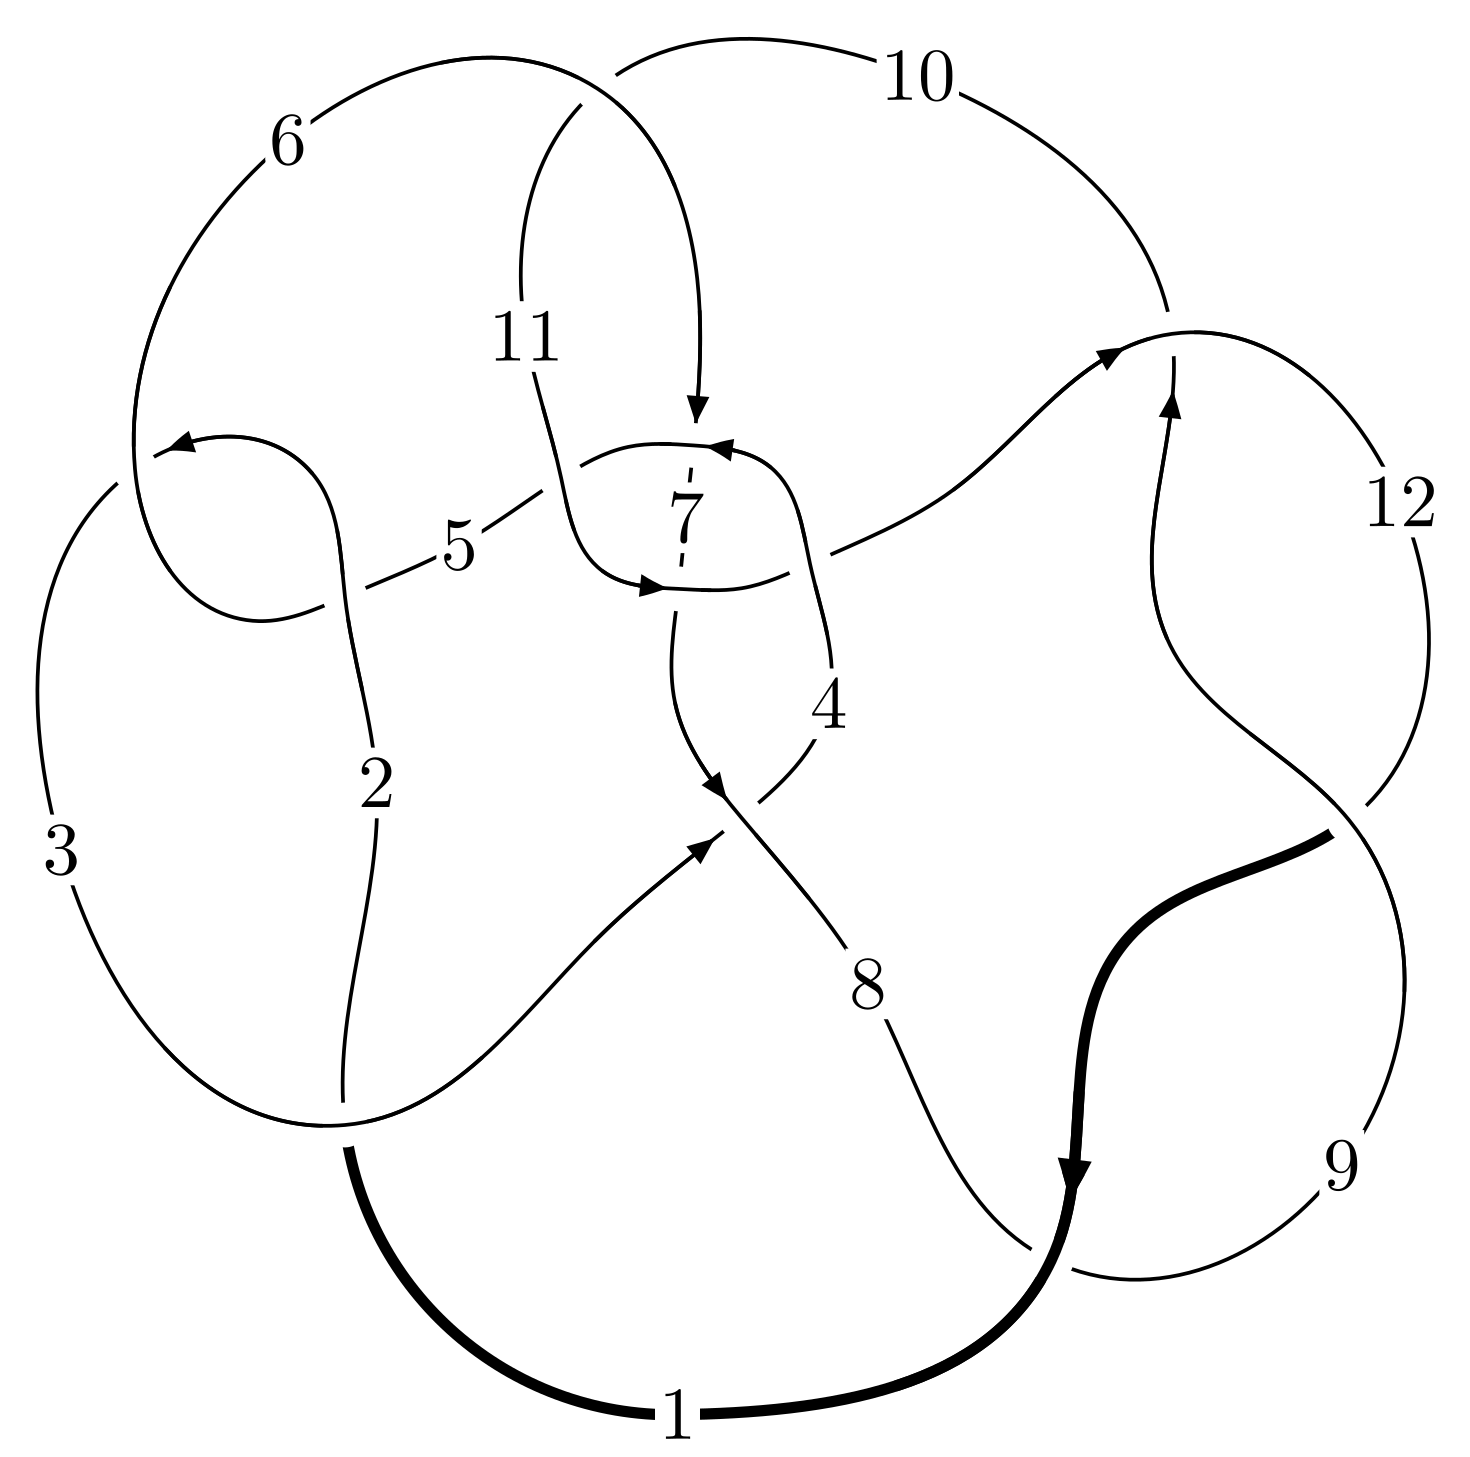
\includegraphics[width=112pt]{../../../GIT/diagram.site/Diagrams/png/2413_12n_0324.png}\\
\ \ \ A knot diagram\footnotemark}&
\allowdisplaybreaks
\textbf{Linearized knot diagam} \\
\cline{2-2}
 &
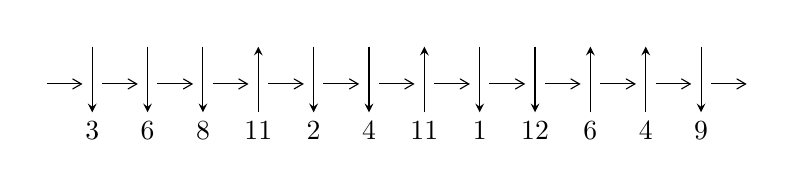
\begin{tikzpicture}[x=20pt, y=17pt]
	% nodes
	\node (C0) at (0, 0) {};
	\node (C1) at (1, 0) {};
	\node (C1U) at (1, +1) {};
	\node (C1D) at (1, -1) {3};

	\node (C2) at (2, 0) {};
	\node (C2U) at (2, +1) {};
	\node (C2D) at (2, -1) {6};

	\node (C3) at (3, 0) {};
	\node (C3U) at (3, +1) {};
	\node (C3D) at (3, -1) {8};

	\node (C4) at (4, 0) {};
	\node (C4U) at (4, +1) {};
	\node (C4D) at (4, -1) {11};

	\node (C5) at (5, 0) {};
	\node (C5U) at (5, +1) {};
	\node (C5D) at (5, -1) {2};

	\node (C6) at (6, 0) {};
	\node (C6U) at (6, +1) {};
	\node (C6D) at (6, -1) {4};

	\node (C7) at (7, 0) {};
	\node (C7U) at (7, +1) {};
	\node (C7D) at (7, -1) {11};

	\node (C8) at (8, 0) {};
	\node (C8U) at (8, +1) {};
	\node (C8D) at (8, -1) {1};

	\node (C9) at (9, 0) {};
	\node (C9U) at (9, +1) {};
	\node (C9D) at (9, -1) {12};

	\node (C10) at (10, 0) {};
	\node (C10U) at (10, +1) {};
	\node (C10D) at (10, -1) {6};

	\node (C11) at (11, 0) {};
	\node (C11U) at (11, +1) {};
	\node (C11D) at (11, -1) {4};

	\node (C12) at (12, 0) {};
	\node (C12U) at (12, +1) {};
	\node (C12D) at (12, -1) {9};
	\node (C13) at (13, 0) {};

	% arrows
	\draw[->,>={angle 60}]
	(C0) edge (C1) (C1) edge (C2) (C2) edge (C3) (C3) edge (C4) (C4) edge (C5) (C5) edge (C6) (C6) edge (C7) (C7) edge (C8) (C8) edge (C9) (C9) edge (C10) (C10) edge (C11) (C11) edge (C12) (C12) edge (C13) ;	\draw[->,>=stealth]
	(C1U) edge (C1D) (C2U) edge (C2D) (C3U) edge (C3D) (C4D) edge (C4U) (C5U) edge (C5D) (C6U) edge (C6D) (C7D) edge (C7U) (C8U) edge (C8D) (C9U) edge (C9D) (C10D) edge (C10U) (C11D) edge (C11U) (C12U) edge (C12D) ;
	\end{tikzpicture} \\
\hhline{~~} \\& 
\textbf{Solving Sequence} \\ \cline{2-2} 
 &
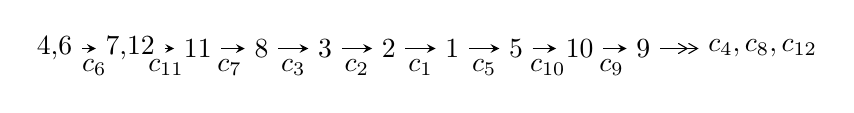
\begin{tikzpicture}[x=23pt, y=7pt]
	% node
	\node (A0) at (-1/8, 0) {4,6};
	\node (A1) at (17/16, 0) {7,12};
	\node (A2) at (17/8, 0) {11};
	\node (A3) at (25/8, 0) {8};
	\node (A4) at (33/8, 0) {3};
	\node (A5) at (41/8, 0) {2};
	\node (A6) at (49/8, 0) {1};
	\node (A7) at (57/8, 0) {5};
	\node (A8) at (65/8, 0) {10};
	\node (A9) at (73/8, 0) {9};
	\node (C1) at (1/2, -1) {$c_{6}$};
	\node (C2) at (13/8, -1) {$c_{11}$};
	\node (C3) at (21/8, -1) {$c_{7}$};
	\node (C4) at (29/8, -1) {$c_{3}$};
	\node (C5) at (37/8, -1) {$c_{2}$};
	\node (C6) at (45/8, -1) {$c_{1}$};
	\node (C7) at (53/8, -1) {$c_{5}$};
	\node (C8) at (61/8, -1) {$c_{10}$};
	\node (C9) at (69/8, -1) {$c_{9}$};
	\node (A10) at (11, 0) {$c_{4},c_{8},c_{12}$};

	% edge
	\draw[->,>=stealth]	
	(A0) edge (A1) (A1) edge (A2) (A2) edge (A3) (A3) edge (A4) (A4) edge (A5) (A5) edge (A6) (A6) edge (A7) (A7) edge (A8) (A8) edge (A9) ;
	\draw[->>,>={angle 60}]	
	(A9) edge (A10);
\end{tikzpicture} \\ 

\end{tabular} \\

\footnotetext{
The image of knot diagram is generated by the software ``\textbf{Draw programme}" developed by Andrew Bartholomew(\url{http://www.layer8.co.uk/maths/draw/index.htm\#Running-draw}), where we modified some parts for our purpose(\url{https://github.com/CATsTAILs/LinksPainter}).
}\phantom \\ \newline 
\centering \textbf{Ideals for irreducible components\footnotemark of $X_{\text{par}}$} 
 
\begin{align*}
I^u_{1}&=\langle 
-6.20623\times10^{189} u^{50}+1.91950\times10^{190} u^{49}+\cdots+1.83109\times10^{190} b-2.76698\times10^{190},\\
\phantom{I^u_{1}}&\phantom{= \langle  }6.53118\times10^{190} u^{50}-2.00240\times10^{191} u^{49}+\cdots+1.83109\times10^{190} a+4.17386\times10^{191},\;u^{51}-3 u^{50}+\cdots+21 u+1\rangle \\
I^u_{2}&=\langle 
-15199 u^{17}-83246 u^{16}+\cdots+b-28434,\;13363 u^{17}+74911 u^{16}+\cdots+a+32129,\\
\phantom{I^u_{2}}&\phantom{= \langle  }u^{18}+6 u^{17}+\cdots+16 u+1\rangle \\
\\
\end{align*}
\raggedright * 2 irreducible components of $\dim_{\mathbb{C}}=0$, with total 69 representations.\\
\footnotetext{All coefficients of polynomials are rational numbers. But the coefficients are sometimes approximated in decimal forms when there is not enough margin.}
\newpage
\renewcommand{\arraystretch}{1}
\centering \section*{I. $I^u_{1}= \langle -6.21\times10^{189} u^{50}+1.92\times10^{190} u^{49}+\cdots+1.83\times10^{190} b-2.77\times10^{190},\;6.53\times10^{190} u^{50}-2.00\times10^{191} u^{49}+\cdots+1.83\times10^{190} a+4.17\times10^{191},\;u^{51}-3 u^{50}+\cdots+21 u+1 \rangle$}
\flushleft \textbf{(i) Arc colorings}\\
\begin{tabular}{m{7pt} m{180pt} m{7pt} m{180pt} }
\flushright $a_{4}=$&$\begin{pmatrix}0\\u\end{pmatrix}$ \\
\flushright $a_{6}=$&$\begin{pmatrix}1\\0\end{pmatrix}$ \\
\flushright $a_{7}=$&$\begin{pmatrix}1\\u^2\end{pmatrix}$ \\
\flushright $a_{12}=$&$\begin{pmatrix}-3.56682 u^{50}+10.9355 u^{49}+\cdots-381.856 u-22.7943\\0.338936 u^{50}-1.04828 u^{49}+\cdots+35.0303 u+1.51111\end{pmatrix}$ \\
\flushright $a_{11}=$&$\begin{pmatrix}-3.56682 u^{50}+10.9355 u^{49}+\cdots-381.856 u-22.7943\\0.367596 u^{50}-1.14233 u^{49}+\cdots+33.6608 u+1.27604\end{pmatrix}$ \\
\flushright $a_{8}=$&$\begin{pmatrix}1.31856 u^{50}-4.24593 u^{49}+\cdots+43.2461 u-7.28846\\0.372098 u^{50}-1.15390 u^{49}+\cdots+41.7658 u+3.50605\end{pmatrix}$ \\
\flushright $a_{3}=$&$\begin{pmatrix}2.56187 u^{50}-8.01615 u^{49}+\cdots+312.685 u+11.1314\\-0.123273 u^{50}+0.394024 u^{49}+\cdots-16.0948 u+0.114225\end{pmatrix}$ \\
\flushright $a_{2}=$&$\begin{pmatrix}2.43859 u^{50}-7.62212 u^{49}+\cdots+296.590 u+11.2457\\-0.123273 u^{50}+0.394024 u^{49}+\cdots-16.0948 u+0.114225\end{pmatrix}$ \\
\flushright $a_{1}=$&$\begin{pmatrix}-0.386563 u^{50}+1.15851 u^{49}+\cdots-202.479 u-17.3283\\0.237140 u^{50}-0.750279 u^{49}+\cdots+32.0577 u+2.33690\end{pmatrix}$ \\
\flushright $a_{5}=$&$\begin{pmatrix}-2.62715 u^{50}+8.16557 u^{49}+\cdots-395.092 u-18.3358\\0.245732 u^{50}-0.780842 u^{49}+\cdots+33.6386 u+1.03443\end{pmatrix}$ \\
\flushright $a_{10}=$&$\begin{pmatrix}-3.93442 u^{50}+12.0779 u^{49}+\cdots-415.517 u-24.0704\\0.367596 u^{50}-1.14233 u^{49}+\cdots+33.6608 u+1.27604\end{pmatrix}$ \\
\flushright $a_{9}=$&$\begin{pmatrix}-1.41365 u^{50}+4.64782 u^{49}+\cdots+32.0023 u+3.74234\\-0.0397767 u^{50}+0.116546 u^{49}+\cdots-24.0454 u-1.81099\end{pmatrix}$\\&\end{tabular}
\flushleft \textbf{(ii) Obstruction class $= -1$}\\~\\
\flushleft \textbf{(iii) Cusp Shapes $= -2.64179 u^{50}+8.09527 u^{49}+\cdots-400.109 u-30.6870$}\\~\\
\newpage\renewcommand{\arraystretch}{1}
\flushleft \textbf{(iv) u-Polynomials at the component}\newline \\
\begin{tabular}{m{50pt}|m{274pt}}
Crossings & \hspace{64pt}u-Polynomials at each crossing \\
\hline $$\begin{aligned}c_{1}\end{aligned}$$&$\begin{aligned}
&u^{51}+29 u^{50}+\cdots-31 u+49
\end{aligned}$\\
\hline $$\begin{aligned}c_{2},c_{5}\end{aligned}$$&$\begin{aligned}
&u^{51}+3 u^{50}+\cdots+33 u+7
\end{aligned}$\\
\hline $$\begin{aligned}c_{3}\end{aligned}$$&$\begin{aligned}
&u^{51}+u^{50}+\cdots-133 u+163
\end{aligned}$\\
\hline $$\begin{aligned}c_{4},c_{11}\end{aligned}$$&$\begin{aligned}
&u^{51}- u^{50}+\cdots-3 u+1
\end{aligned}$\\
\hline $$\begin{aligned}c_{6}\end{aligned}$$&$\begin{aligned}
&u^{51}-3 u^{50}+\cdots+21 u+1
\end{aligned}$\\
\hline $$\begin{aligned}c_{7}\end{aligned}$$&$\begin{aligned}
&u^{51}-2 u^{50}+\cdots+6290 u+161
\end{aligned}$\\
\hline $$\begin{aligned}c_{8},c_{9},c_{12}\end{aligned}$$&$\begin{aligned}
&u^{51}-4 u^{50}+\cdots+131 u-29
\end{aligned}$\\
\hline $$\begin{aligned}c_{10}\end{aligned}$$&$\begin{aligned}
&u^{51}+33 u^{49}+\cdots+63366 u+32041
\end{aligned}$\\
\hline
\end{tabular}\\~\\
\newpage\renewcommand{\arraystretch}{1}
\flushleft \textbf{(v) Riley Polynomials at the component}\newline \\
\begin{tabular}{m{50pt}|m{274pt}}
Crossings & \hspace{64pt}Riley Polynomials at each crossing \\
\hline $$\begin{aligned}c_{1}\end{aligned}$$&$\begin{aligned}
&y^{51}- y^{50}+\cdots+295745 y-2401
\end{aligned}$\\
\hline $$\begin{aligned}c_{2},c_{5}\end{aligned}$$&$\begin{aligned}
&y^{51}-29 y^{50}+\cdots-31 y-49
\end{aligned}$\\
\hline $$\begin{aligned}c_{3}\end{aligned}$$&$\begin{aligned}
&y^{51}+19 y^{50}+\cdots-159329 y-26569
\end{aligned}$\\
\hline $$\begin{aligned}c_{4},c_{11}\end{aligned}$$&$\begin{aligned}
&y^{51}+67 y^{50}+\cdots+111 y-1
\end{aligned}$\\
\hline $$\begin{aligned}c_{6}\end{aligned}$$&$\begin{aligned}
&y^{51}-87 y^{50}+\cdots-61 y-1
\end{aligned}$\\
\hline $$\begin{aligned}c_{7}\end{aligned}$$&$\begin{aligned}
&y^{51}+68 y^{50}+\cdots+46092006 y-25921
\end{aligned}$\\
\hline $$\begin{aligned}c_{8},c_{9},c_{12}\end{aligned}$$&$\begin{aligned}
&y^{51}+46 y^{50}+\cdots+14783 y-841
\end{aligned}$\\
\hline $$\begin{aligned}c_{10}\end{aligned}$$&$\begin{aligned}
&y^{51}+66 y^{50}+\cdots-134123626 y-1026625681
\end{aligned}$\\
\hline
\end{tabular}\\~\\
\newpage\flushleft \textbf{(vi) Complex Volumes and Cusp Shapes}
$$\begin{array}{c|c|c}  
\text{Solutions to }I^u_{1}& \I (\text{vol} + \sqrt{-1}CS) & \text{Cusp shape}\\
 \hline 
\begin{aligned}
u &= \phantom{-}0.438854 + 0.881387 I \\
a &= \phantom{-}0.802989 + 0.488950 I \\
b &= \phantom{-}1.46263 + 0.44970 I\end{aligned}
 & \phantom{-}2.55303 + 5.62854 I & \phantom{-0.000000 } 0 \\ \hline\begin{aligned}
u &= \phantom{-}0.438854 - 0.881387 I \\
a &= \phantom{-}0.802989 - 0.488950 I \\
b &= \phantom{-}1.46263 - 0.44970 I\end{aligned}
 & \phantom{-}2.55303 - 5.62854 I & \phantom{-0.000000 } 0 \\ \hline\begin{aligned}
u &= \phantom{-}0.786917 + 0.547490 I \\
a &= \phantom{-}1.231510 + 0.622312 I \\
b &= -0.561675 - 0.635936 I\end{aligned}
 & \phantom{-}5.38314 + 2.25660 I & \phantom{-0.000000 } 0 \\ \hline\begin{aligned}
u &= \phantom{-}0.786917 - 0.547490 I \\
a &= \phantom{-}1.231510 - 0.622312 I \\
b &= -0.561675 + 0.635936 I\end{aligned}
 & \phantom{-}5.38314 - 2.25660 I & \phantom{-0.000000 } 0 \\ \hline\begin{aligned}
u &= -0.969635 + 0.549105 I \\
a &= \phantom{-}0.592870 - 0.730545 I \\
b &= \phantom{-}1.099540 + 0.169847 I\end{aligned}
 & \phantom{-}2.80334 + 0.19977 I & \phantom{-0.000000 } 0 \\ \hline\begin{aligned}
u &= -0.969635 - 0.549105 I \\
a &= \phantom{-}0.592870 + 0.730545 I \\
b &= \phantom{-}1.099540 - 0.169847 I\end{aligned}
 & \phantom{-}2.80334 - 0.19977 I & \phantom{-0.000000 } 0 \\ \hline\begin{aligned}
u &= -0.258956 + 1.084080 I \\
a &= -0.0078550 + 0.1186930 I \\
b &= \phantom{-}0.680266 + 0.175141 I\end{aligned}
 & \phantom{-}2.08270 + 2.42338 I & \phantom{-0.000000 } 0 \\ \hline\begin{aligned}
u &= -0.258956 - 1.084080 I \\
a &= -0.0078550 - 0.1186930 I \\
b &= \phantom{-}0.680266 - 0.175141 I\end{aligned}
 & \phantom{-}2.08270 - 2.42338 I & \phantom{-0.000000 } 0 \\ \hline\begin{aligned}
u &= -0.877771 + 0.053196 I \\
a &= \phantom{-}1.06003 - 0.99974 I \\
b &= -0.050000 + 0.341986 I\end{aligned}
 & \phantom{-}2.86052 + 0.92213 I & -4.00000 + 0. I\phantom{ +0.000000I} \\ \hline\begin{aligned}
u &= -0.877771 - 0.053196 I \\
a &= \phantom{-}1.06003 + 0.99974 I \\
b &= -0.050000 - 0.341986 I\end{aligned}
 & \phantom{-}2.86052 - 0.92213 I & -4.00000 + 0. I\phantom{ +0.000000I}\\
 \hline 
 \end{array}$$\newpage$$\begin{array}{c|c|c}  
\text{Solutions to }I^u_{1}& \I (\text{vol} + \sqrt{-1}CS) & \text{Cusp shape}\\
 \hline 
\begin{aligned}
u &= \phantom{-}0.077227 + 0.787735 I \\
a &= -1.39631 + 0.29538 I \\
b &= \phantom{-}0.405257 - 0.172699 I\end{aligned}
 & -1.082690 - 0.753222 I & -8.27224 - 0.58913 I \\ \hline\begin{aligned}
u &= \phantom{-}0.077227 - 0.787735 I \\
a &= -1.39631 - 0.29538 I \\
b &= \phantom{-}0.405257 + 0.172699 I\end{aligned}
 & -1.082690 + 0.753222 I & -8.27224 + 0.58913 I \\ \hline\begin{aligned}
u &= -0.371822 + 0.643704 I \\
a &= -1.319030 + 0.489182 I \\
b &= -1.058190 - 0.552894 I\end{aligned}
 & -1.31122 + 2.27509 I & -10.03353 - 3.12250 I \\ \hline\begin{aligned}
u &= -0.371822 - 0.643704 I \\
a &= -1.319030 - 0.489182 I \\
b &= -1.058190 + 0.552894 I\end{aligned}
 & -1.31122 - 2.27509 I & -10.03353 + 3.12250 I \\ \hline\begin{aligned}
u &= \phantom{-}0.415418 + 1.187680 I \\
a &= \phantom{-}0.210614 + 0.007241 I \\
b &= -0.711873 - 0.851088 I\end{aligned}
 & \phantom{-}7.01209 + 0.55331 I & \phantom{-0.000000 } 0 \\ \hline\begin{aligned}
u &= \phantom{-}0.415418 - 1.187680 I \\
a &= \phantom{-}0.210614 - 0.007241 I \\
b &= -0.711873 + 0.851088 I\end{aligned}
 & \phantom{-}7.01209 - 0.55331 I & \phantom{-0.000000 } 0 \\ \hline\begin{aligned}
u &= -0.851182 + 0.945181 I \\
a &= \phantom{-}0.492401 - 0.719354 I \\
b &= -0.574356 + 0.893531 I\end{aligned}
 & \phantom{-}1.61849 - 3.97257 I & \phantom{-0.000000 } 0 \\ \hline\begin{aligned}
u &= -0.851182 - 0.945181 I \\
a &= \phantom{-}0.492401 + 0.719354 I \\
b &= -0.574356 - 0.893531 I\end{aligned}
 & \phantom{-}1.61849 + 3.97257 I & \phantom{-0.000000 } 0 \\ \hline\begin{aligned}
u &= -0.654550\phantom{ +0.000000I} \\
a &= -0.815626\phantom{ +0.000000I} \\
b &= -0.0235623\phantom{ +0.000000I}\end{aligned}
 & -1.51224\phantom{ +0.000000I} & -6.39690\phantom{ +0.000000I} \\ \hline\begin{aligned}
u &= -0.61210 + 1.42769 I \\
a &= -0.0766712 - 0.0666805 I \\
b &= -0.855685 + 0.583788 I\end{aligned}
 & \phantom{-}5.29873 + 5.39295 I & \phantom{-0.000000 } 0\\
 \hline 
 \end{array}$$\newpage$$\begin{array}{c|c|c}  
\text{Solutions to }I^u_{1}& \I (\text{vol} + \sqrt{-1}CS) & \text{Cusp shape}\\
 \hline 
\begin{aligned}
u &= -0.61210 - 1.42769 I \\
a &= -0.0766712 + 0.0666805 I \\
b &= -0.855685 - 0.583788 I\end{aligned}
 & \phantom{-}5.29873 - 5.39295 I & \phantom{-0.000000 } 0 \\ \hline\begin{aligned}
u &= \phantom{-}0.244067 + 0.211790 I \\
a &= \phantom{-}3.58624 - 0.14006 I \\
b &= -0.172244 - 0.891038 I\end{aligned}
 & \phantom{-}6.22807 + 3.03641 I & -0.15194 - 4.08278 I \\ \hline\begin{aligned}
u &= \phantom{-}0.244067 - 0.211790 I \\
a &= \phantom{-}3.58624 + 0.14006 I \\
b &= -0.172244 + 0.891038 I\end{aligned}
 & \phantom{-}6.22807 - 3.03641 I & -0.15194 + 4.08278 I \\ \hline\begin{aligned}
u &= -0.052211 + 0.243333 I \\
a &= -1.65333 + 1.57397 I \\
b &= \phantom{-}0.032030 + 0.489627 I\end{aligned}
 & -0.123994 + 1.016060 I & -2.35884 - 6.62848 I \\ \hline\begin{aligned}
u &= -0.052211 - 0.243333 I \\
a &= -1.65333 - 1.57397 I \\
b &= \phantom{-}0.032030 - 0.489627 I\end{aligned}
 & -0.123994 - 1.016060 I & -2.35884 + 6.62848 I \\ \hline\begin{aligned}
u &= -0.153372 + 0.111375 I \\
a &= \phantom{-}2.84799 + 0.60731 I \\
b &= \phantom{-}0.517369 + 1.121390 I\end{aligned}
 & -1.19162 + 1.61010 I & -0.97639 + 4.58807 I \\ \hline\begin{aligned}
u &= -0.153372 - 0.111375 I \\
a &= \phantom{-}2.84799 - 0.60731 I \\
b &= \phantom{-}0.517369 - 1.121390 I\end{aligned}
 & -1.19162 - 1.61010 I & -0.97639 - 4.58807 I \\ \hline\begin{aligned}
u &= \phantom{-}0.007539 + 0.153031 I \\
a &= -5.36804 + 7.36280 I \\
b &= \phantom{-}0.090420 - 0.966899 I\end{aligned}
 & \phantom{-}3.36883 + 8.08804 I & -4.16795 - 6.45391 I \\ \hline\begin{aligned}
u &= \phantom{-}0.007539 - 0.153031 I \\
a &= -5.36804 - 7.36280 I \\
b &= \phantom{-}0.090420 + 0.966899 I\end{aligned}
 & \phantom{-}3.36883 - 8.08804 I & -4.16795 + 6.45391 I \\ \hline\begin{aligned}
u &= -0.0981206 + 0.0761409 I \\
a &= -2.13969 - 7.63551 I \\
b &= -0.180819 + 1.098890 I\end{aligned}
 & -2.72745 + 3.79308 I & -7.08139 - 6.39060 I\\
 \hline 
 \end{array}$$\newpage$$\begin{array}{c|c|c}  
\text{Solutions to }I^u_{1}& \I (\text{vol} + \sqrt{-1}CS) & \text{Cusp shape}\\
 \hline 
\begin{aligned}
u &= -0.0981206 - 0.0761409 I \\
a &= -2.13969 + 7.63551 I \\
b &= -0.180819 - 1.098890 I\end{aligned}
 & -2.72745 - 3.79308 I & -7.08139 + 6.39060 I \\ \hline\begin{aligned}
u &= \phantom{-}2.03972 + 0.34818 I \\
a &= -0.167321 - 0.858121 I \\
b &= \phantom{-}0.24093 + 2.09041 I\end{aligned}
 & -7.53123 - 4.56112 I & \phantom{-0.000000 } 0 \\ \hline\begin{aligned}
u &= \phantom{-}2.03972 - 0.34818 I \\
a &= -0.167321 + 0.858121 I \\
b &= \phantom{-}0.24093 - 2.09041 I\end{aligned}
 & -7.53123 + 4.56112 I & \phantom{-0.000000 } 0 \\ \hline\begin{aligned}
u &= \phantom{-}2.11807 + 0.20852 I \\
a &= \phantom{-}0.111419 + 0.870257 I \\
b &= \phantom{-}0.53451 - 1.37759 I\end{aligned}
 & -9.45111 - 1.99019 I & \phantom{-0.000000 } 0 \\ \hline\begin{aligned}
u &= \phantom{-}2.11807 - 0.20852 I \\
a &= \phantom{-}0.111419 - 0.870257 I \\
b &= \phantom{-}0.53451 + 1.37759 I\end{aligned}
 & -9.45111 + 1.99019 I & \phantom{-0.000000 } 0 \\ \hline\begin{aligned}
u &= \phantom{-}2.14783 + 0.07904 I \\
a &= \phantom{-}0.027350 + 0.853045 I \\
b &= -0.32027 - 1.82960 I\end{aligned}
 & -12.63600 - 1.06445 I & \phantom{-0.000000 } 0 \\ \hline\begin{aligned}
u &= \phantom{-}2.14783 - 0.07904 I \\
a &= \phantom{-}0.027350 - 0.853045 I \\
b &= -0.32027 + 1.82960 I\end{aligned}
 & -12.63600 + 1.06445 I & \phantom{-0.000000 } 0 \\ \hline\begin{aligned}
u &= \phantom{-}2.09075 + 0.50266 I \\
a &= -0.344685 - 0.686017 I \\
b &= \phantom{-}0.07196 + 1.68618 I\end{aligned}
 & -7.39570 + 2.33947 I & \phantom{-0.000000 } 0 \\ \hline\begin{aligned}
u &= \phantom{-}2.09075 - 0.50266 I \\
a &= -0.344685 + 0.686017 I \\
b &= \phantom{-}0.07196 - 1.68618 I\end{aligned}
 & -7.39570 - 2.33947 I & \phantom{-0.000000 } 0 \\ \hline\begin{aligned}
u &= -2.16315 + 0.30765 I \\
a &= -0.100617 + 0.731102 I \\
b &= -0.04164 - 2.25566 I\end{aligned}
 & -5.84292 + 0.77536 I & \phantom{-0.000000 } 0\\
 \hline 
 \end{array}$$\newpage$$\begin{array}{c|c|c}  
\text{Solutions to }I^u_{1}& \I (\text{vol} + \sqrt{-1}CS) & \text{Cusp shape}\\
 \hline 
\begin{aligned}
u &= -2.16315 - 0.30765 I \\
a &= -0.100617 - 0.731102 I \\
b &= -0.04164 + 2.25566 I\end{aligned}
 & -5.84292 - 0.77536 I & \phantom{-0.000000 } 0 \\ \hline\begin{aligned}
u &= -2.24014 + 0.35466 I \\
a &= \phantom{-}0.021038 - 0.775624 I \\
b &= \phantom{-}0.69469 + 1.78191 I\end{aligned}
 & -2.40989 + 7.37799 I & \phantom{-0.000000 } 0 \\ \hline\begin{aligned}
u &= -2.24014 - 0.35466 I \\
a &= \phantom{-}0.021038 + 0.775624 I \\
b &= \phantom{-}0.69469 - 1.78191 I\end{aligned}
 & -2.40989 - 7.37799 I & \phantom{-0.000000 } 0 \\ \hline\begin{aligned}
u &= -2.22716 + 0.44704 I \\
a &= -0.192890 + 0.625827 I \\
b &= -0.19805 - 1.86310 I\end{aligned}
 & -5.46694 + 1.77932 I & \phantom{-0.000000 } 0 \\ \hline\begin{aligned}
u &= -2.22716 - 0.44704 I \\
a &= -0.192890 - 0.625827 I \\
b &= -0.19805 + 1.86310 I\end{aligned}
 & -5.46694 - 1.77932 I & \phantom{-0.000000 } 0 \\ \hline\begin{aligned}
u &= -2.28681 + 0.02141 I \\
a &= \phantom{-}0.069554 + 0.723390 I \\
b &= -0.35195 - 1.92261 I\end{aligned}
 & -7.57553 + 3.10359 I & \phantom{-0.000000 } 0 \\ \hline\begin{aligned}
u &= -2.28681 - 0.02141 I \\
a &= \phantom{-}0.069554 - 0.723390 I \\
b &= -0.35195 + 1.92261 I\end{aligned}
 & -7.57553 - 3.10359 I & \phantom{-0.000000 } 0 \\ \hline\begin{aligned}
u &= \phantom{-}2.29535 + 0.30641 I \\
a &= -0.050327 + 0.786971 I \\
b &= \phantom{-}0.58797 - 1.96230 I\end{aligned}
 & -5.2040 - 14.0594 I & \phantom{-0.000000 } 0 \\ \hline\begin{aligned}
u &= \phantom{-}2.29535 - 0.30641 I \\
a &= -0.050327 - 0.786971 I \\
b &= \phantom{-}0.58797 + 1.96230 I\end{aligned}
 & -5.2040 + 14.0594 I & \phantom{-0.000000 } 0 \\ \hline\begin{aligned}
u &= \phantom{-}2.32797 + 0.06553 I \\
a &= \phantom{-}0.170579 + 0.730407 I \\
b &= -0.32905 - 1.92841 I\end{aligned}
 & -10.44840 + 8.57270 I & \phantom{-0.000000 } 0\\
 \hline 
 \end{array}$$\newpage$$\begin{array}{c|c|c}  
\text{Solutions to }I^u_{1}& \I (\text{vol} + \sqrt{-1}CS) & \text{Cusp shape}\\
 \hline 
\begin{aligned}
u &= \phantom{-}2.32797 - 0.06553 I \\
a &= \phantom{-}0.170579 - 0.730407 I \\
b &= -0.32905 + 1.92841 I\end{aligned}
 & -10.44840 - 8.57270 I & \phantom{-0.000000 } 0\\
 \hline 
 \end{array}$$\newpage\newpage\renewcommand{\arraystretch}{1}
\centering \section*{II. $I^u_{2}= \langle -15199 u^{17}-83246 u^{16}+\cdots+b-28434,\;13363 u^{17}+74911 u^{16}+\cdots+a+32129,\;u^{18}+6 u^{17}+\cdots+16 u+1 \rangle$}
\flushleft \textbf{(i) Arc colorings}\\
\begin{tabular}{m{7pt} m{180pt} m{7pt} m{180pt} }
\flushright $a_{4}=$&$\begin{pmatrix}0\\u\end{pmatrix}$ \\
\flushright $a_{6}=$&$\begin{pmatrix}1\\0\end{pmatrix}$ \\
\flushright $a_{7}=$&$\begin{pmatrix}1\\u^2\end{pmatrix}$ \\
\flushright $a_{12}=$&$\begin{pmatrix}-13363 u^{17}-74911 u^{16}+\cdots-440720 u-32129\\15199 u^{17}+83246 u^{16}+\cdots+403343 u+28434\end{pmatrix}$ \\
\flushright $a_{11}=$&$\begin{pmatrix}-13363 u^{17}-74911 u^{16}+\cdots-440720 u-32129\\13235 u^{17}+72159 u^{16}+\cdots+332434 u+23167\end{pmatrix}$ \\
\flushright $a_{8}=$&$\begin{pmatrix}-16 u^{17}-94 u^{16}+\cdots-1251 u-125\\16384 u^{17}+90112 u^{16}+\cdots+458752 u+32767\end{pmatrix}$ \\
\flushright $a_{3}=$&$\begin{pmatrix}-93 u^{17}-558 u^{16}+\cdots-6698 u-592\\- u^{17}-6 u^{16}+\cdots-115 u-15\end{pmatrix}$ \\
\flushright $a_{2}=$&$\begin{pmatrix}-94 u^{17}-564 u^{16}+\cdots-6813 u-607\\- u^{17}-6 u^{16}+\cdots-115 u-15\end{pmatrix}$ \\
\flushright $a_{1}=$&$\begin{pmatrix}1589 u^{17}+9128 u^{16}+\cdots+70803 u+5487\\95 u^{17}+557 u^{16}+\cdots+5933 u+515\end{pmatrix}$ \\
\flushright $a_{5}=$&$\begin{pmatrix}-513 u^{17}-2984 u^{16}+\cdots-27756 u-2291\\-14 u^{17}-83 u^{16}+\cdots-1120 u-110\end{pmatrix}$ \\
\flushright $a_{10}=$&$\begin{pmatrix}-26598 u^{17}-147070 u^{16}+\cdots-773154 u-55296\\13235 u^{17}+72159 u^{16}+\cdots+332434 u+23167\end{pmatrix}$ \\
\flushright $a_{9}=$&$\begin{pmatrix}-24899 u^{17}-137296 u^{16}+\cdots-695183 u-49170\\13235 u^{17}+72171 u^{16}+\cdots+333330 u+23261\end{pmatrix}$\\&\end{tabular}
\flushleft \textbf{(ii) Obstruction class $= 1$}\\~\\
\flushleft \textbf{(iii) Cusp Shapes $= 96456 u^{17}+526448 u^{16}+968430 u^{15}-43279 u^{14}-4993167 u^{13}-14847798 u^{12}-21267959 u^{11}-7843139 u^{10}+43624726 u^9+131260980 u^8+221053250 u^7+262385524 u^6+225728266 u^5+138033421 u^4+57916786 u^3+15777654 u^2+2510027 u+177106$}\\~\\
\newpage\renewcommand{\arraystretch}{1}
\flushleft \textbf{(iv) u-Polynomials at the component}\newline \\
\begin{tabular}{m{50pt}|m{274pt}}
Crossings & \hspace{64pt}u-Polynomials at each crossing \\
\hline $$\begin{aligned}c_{1}\end{aligned}$$&$\begin{aligned}
&u^{18}-12 u^{17}+\cdots-12 u+1
\end{aligned}$\\
\hline $$\begin{aligned}c_{2}\end{aligned}$$&$\begin{aligned}
&u^{18}+2 u^{17}+\cdots+2 u+1
\end{aligned}$\\
\hline $$\begin{aligned}c_{3}\end{aligned}$$&$\begin{aligned}
&u^{18}+6 u^{16}+\cdots-6 u+1
\end{aligned}$\\
\hline $$\begin{aligned}c_{4}\end{aligned}$$&$\begin{aligned}
&u^{18}+10 u^{16}+\cdots+17 u^2+1
\end{aligned}$\\
\hline $$\begin{aligned}c_{5}\end{aligned}$$&$\begin{aligned}
&u^{18}-2 u^{17}+\cdots-2 u+1
\end{aligned}$\\
\hline $$\begin{aligned}c_{6}\end{aligned}$$&$\begin{aligned}
&u^{18}+6 u^{17}+\cdots+16 u+1
\end{aligned}$\\
\hline $$\begin{aligned}c_{7}\end{aligned}$$&$\begin{aligned}
&u^{18}- u^{17}+\cdots- u+1
\end{aligned}$\\
\hline $$\begin{aligned}c_{8},c_{9}\end{aligned}$$&$\begin{aligned}
&u^{18}-3 u^{17}+\cdots-4 u+1
\end{aligned}$\\
\hline $$\begin{aligned}c_{10}\end{aligned}$$&$\begin{aligned}
&u^{18}+u^{17}+\cdots+u+1
\end{aligned}$\\
\hline $$\begin{aligned}c_{11}\end{aligned}$$&$\begin{aligned}
&u^{18}+10 u^{16}+\cdots+17 u^2+1
\end{aligned}$\\
\hline $$\begin{aligned}c_{12}\end{aligned}$$&$\begin{aligned}
&u^{18}+3 u^{17}+\cdots+4 u+1
\end{aligned}$\\
\hline
\end{tabular}\\~\\
\newpage\renewcommand{\arraystretch}{1}
\flushleft \textbf{(v) Riley Polynomials at the component}\newline \\
\begin{tabular}{m{50pt}|m{274pt}}
Crossings & \hspace{64pt}Riley Polynomials at each crossing \\
\hline $$\begin{aligned}c_{1}\end{aligned}$$&$\begin{aligned}
&y^{18}-8 y^{16}+\cdots-8 y+1
\end{aligned}$\\
\hline $$\begin{aligned}c_{2},c_{5}\end{aligned}$$&$\begin{aligned}
&y^{18}-12 y^{17}+\cdots-12 y+1
\end{aligned}$\\
\hline $$\begin{aligned}c_{3}\end{aligned}$$&$\begin{aligned}
&y^{18}+12 y^{17}+\cdots-6 y+1
\end{aligned}$\\
\hline $$\begin{aligned}c_{4},c_{11}\end{aligned}$$&$\begin{aligned}
&y^{18}+20 y^{17}+\cdots+34 y+1
\end{aligned}$\\
\hline $$\begin{aligned}c_{6}\end{aligned}$$&$\begin{aligned}
&y^{18}-10 y^{17}+\cdots-26 y+1
\end{aligned}$\\
\hline $$\begin{aligned}c_{7}\end{aligned}$$&$\begin{aligned}
&y^{18}+13 y^{17}+\cdots-5 y+1
\end{aligned}$\\
\hline $$\begin{aligned}c_{8},c_{9},c_{12}\end{aligned}$$&$\begin{aligned}
&y^{18}+19 y^{17}+\cdots+34 y+1
\end{aligned}$\\
\hline $$\begin{aligned}c_{10}\end{aligned}$$&$\begin{aligned}
&y^{18}+7 y^{17}+\cdots-9 y+1
\end{aligned}$\\
\hline
\end{tabular}\\~\\
\newpage\flushleft \textbf{(vi) Complex Volumes and Cusp Shapes}
$$\begin{array}{c|c|c}  
\text{Solutions to }I^u_{2}& \I (\text{vol} + \sqrt{-1}CS) & \text{Cusp shape}\\
 \hline 
\begin{aligned}
u &= -0.642965 + 1.138500 I \\
a &= -0.809556 - 0.016966 I \\
b &= -0.104175 - 0.781798 I\end{aligned}
 & \phantom{-}6.64743 - 1.50205 I & \phantom{-0.000000 } 0 \\ \hline\begin{aligned}
u &= -0.642965 - 1.138500 I \\
a &= -0.809556 + 0.016966 I \\
b &= -0.104175 + 0.781798 I\end{aligned}
 & \phantom{-}6.64743 + 1.50205 I & \phantom{-0.000000 } 0 \\ \hline\begin{aligned}
u &= -0.586828 + 0.199257 I \\
a &= -1.39182 + 1.34971 I \\
b &= \phantom{-}0.880804 - 0.592549 I\end{aligned}
 & \phantom{-}6.10975 - 2.66232 I & \phantom{-}2.22310 + 5.30109 I \\ \hline\begin{aligned}
u &= -0.586828 - 0.199257 I \\
a &= -1.39182 - 1.34971 I \\
b &= \phantom{-}0.880804 + 0.592549 I\end{aligned}
 & \phantom{-}6.10975 + 2.66232 I & \phantom{-}2.22310 - 5.30109 I \\ \hline\begin{aligned}
u &= \phantom{-}0.12002 + 1.43750 I \\
a &= -0.563405 + 0.344470 I \\
b &= -0.585179 + 0.241540 I\end{aligned}
 & \phantom{-}5.29038 + 6.84249 I & \phantom{-0.000000 } 0 \\ \hline\begin{aligned}
u &= \phantom{-}0.12002 - 1.43750 I \\
a &= -0.563405 - 0.344470 I \\
b &= -0.585179 - 0.241540 I\end{aligned}
 & \phantom{-}5.29038 - 6.84249 I & \phantom{-0.000000 } 0 \\ \hline\begin{aligned}
u &= -0.533613 + 0.020740 I \\
a &= \phantom{-}0.029715 - 0.541718 I \\
b &= -0.493263 + 0.922302 I\end{aligned}
 & -1.38579 - 2.18536 I & -5.51806 + 7.75600 I \\ \hline\begin{aligned}
u &= -0.533613 - 0.020740 I \\
a &= \phantom{-}0.029715 + 0.541718 I \\
b &= -0.493263 - 0.922302 I\end{aligned}
 & -1.38579 + 2.18536 I & -5.51806 - 7.75600 I \\ \hline\begin{aligned}
u &= -0.483081 + 0.122779 I \\
a &= \phantom{-}0.22219 - 1.99454 I \\
b &= -0.880434 + 0.479597 I\end{aligned}
 & -0.12655 - 1.97803 I & -2.99483 + 2.76111 I \\ \hline\begin{aligned}
u &= -0.483081 - 0.122779 I \\
a &= \phantom{-}0.22219 + 1.99454 I \\
b &= -0.880434 - 0.479597 I\end{aligned}
 & -0.12655 + 1.97803 I & -2.99483 - 2.76111 I\\
 \hline 
 \end{array}$$\newpage$$\begin{array}{c|c|c}  
\text{Solutions to }I^u_{2}& \I (\text{vol} + \sqrt{-1}CS) & \text{Cusp shape}\\
 \hline 
\begin{aligned}
u &= -0.30885 + 1.52377 I \\
a &= \phantom{-}0.446642 - 0.096804 I \\
b &= \phantom{-}0.487692 + 0.273624 I\end{aligned}
 & \phantom{-}1.24279 + 2.46392 I & \phantom{-0.000000 } 0 \\ \hline\begin{aligned}
u &= -0.30885 - 1.52377 I \\
a &= \phantom{-}0.446642 + 0.096804 I \\
b &= \phantom{-}0.487692 - 0.273624 I\end{aligned}
 & \phantom{-}1.24279 - 2.46392 I & \phantom{-0.000000 } 0 \\ \hline\begin{aligned}
u &= -0.413975 + 0.113860 I \\
a &= \phantom{-}0.76007 + 3.22513 I \\
b &= \phantom{-}0.849984 - 0.349023 I\end{aligned}
 & \phantom{-}3.66442 - 2.08584 I & -0.82702 + 3.16487 I \\ \hline\begin{aligned}
u &= -0.413975 - 0.113860 I \\
a &= \phantom{-}0.76007 - 3.22513 I \\
b &= \phantom{-}0.849984 + 0.349023 I\end{aligned}
 & \phantom{-}3.66442 + 2.08584 I & -0.82702 - 3.16487 I \\ \hline\begin{aligned}
u &= \phantom{-}2.09428 + 0.29167 I \\
a &= \phantom{-}0.161339 + 0.853648 I \\
b &= \phantom{-}0.18266 - 1.56242 I\end{aligned}
 & -10.12730 - 0.84676 I & \phantom{-0.000000 } 0 \\ \hline\begin{aligned}
u &= \phantom{-}2.09428 - 0.29167 I \\
a &= \phantom{-}0.161339 - 0.853648 I \\
b &= \phantom{-}0.18266 + 1.56242 I\end{aligned}
 & -10.12730 + 0.84676 I & \phantom{-0.000000 } 0 \\ \hline\begin{aligned}
u &= -2.24499 + 0.38125 I \\
a &= \phantom{-}0.144822 - 0.657660 I \\
b &= \phantom{-}0.16191 + 2.21998 I\end{aligned}
 & -6.38032 + 1.49135 I & \phantom{-0.000000 } 0 \\ \hline\begin{aligned}
u &= -2.24499 - 0.38125 I \\
a &= \phantom{-}0.144822 + 0.657660 I \\
b &= \phantom{-}0.16191 - 2.21998 I\end{aligned}
 & -6.38032 - 1.49135 I & \phantom{-0.000000 } 0\\
 \hline 
 \end{array}$$\newpage
\newpage\renewcommand{\arraystretch}{1}
\centering \section*{ III. u-Polynomials}
\begin{tabular}{m{50pt}|m{274pt}}
Crossings & \hspace{64pt}u-Polynomials at each crossing \\
\hline $$\begin{aligned}c_{1}\end{aligned}$$&$\begin{aligned}
&(u^{18}-12 u^{17}+\cdots-12 u+1)(u^{51}+29 u^{50}+\cdots-31 u+49)
\end{aligned}$\\
\hline $$\begin{aligned}c_{2}\end{aligned}$$&$\begin{aligned}
&(u^{18}+2 u^{17}+\cdots+2 u+1)(u^{51}+3 u^{50}+\cdots+33 u+7)
\end{aligned}$\\
\hline $$\begin{aligned}c_{3}\end{aligned}$$&$\begin{aligned}
&(u^{18}+6 u^{16}+\cdots-6 u+1)(u^{51}+u^{50}+\cdots-133 u+163)
\end{aligned}$\\
\hline $$\begin{aligned}c_{4}\end{aligned}$$&$\begin{aligned}
&(u^{18}+10 u^{16}+\cdots+17 u^2+1)(u^{51}- u^{50}+\cdots-3 u+1)
\end{aligned}$\\
\hline $$\begin{aligned}c_{5}\end{aligned}$$&$\begin{aligned}
&(u^{18}-2 u^{17}+\cdots-2 u+1)(u^{51}+3 u^{50}+\cdots+33 u+7)
\end{aligned}$\\
\hline $$\begin{aligned}c_{6}\end{aligned}$$&$\begin{aligned}
&(u^{18}+6 u^{17}+\cdots+16 u+1)(u^{51}-3 u^{50}+\cdots+21 u+1)
\end{aligned}$\\
\hline $$\begin{aligned}c_{7}\end{aligned}$$&$\begin{aligned}
&(u^{18}- u^{17}+\cdots- u+1)(u^{51}-2 u^{50}+\cdots+6290 u+161)
\end{aligned}$\\
\hline $$\begin{aligned}c_{8},c_{9}\end{aligned}$$&$\begin{aligned}
&(u^{18}-3 u^{17}+\cdots-4 u+1)(u^{51}-4 u^{50}+\cdots+131 u-29)
\end{aligned}$\\
\hline $$\begin{aligned}c_{10}\end{aligned}$$&$\begin{aligned}
&(u^{18}+u^{17}+\cdots+u+1)(u^{51}+33 u^{49}+\cdots+63366 u+32041)
\end{aligned}$\\
\hline $$\begin{aligned}c_{11}\end{aligned}$$&$\begin{aligned}
&(u^{18}+10 u^{16}+\cdots+17 u^2+1)(u^{51}- u^{50}+\cdots-3 u+1)
\end{aligned}$\\
\hline $$\begin{aligned}c_{12}\end{aligned}$$&$\begin{aligned}
&(u^{18}+3 u^{17}+\cdots+4 u+1)(u^{51}-4 u^{50}+\cdots+131 u-29)
\end{aligned}$\\
\hline
\end{tabular}\newpage\renewcommand{\arraystretch}{1}
\centering \section*{ IV. Riley Polynomials}
\begin{tabular}{m{50pt}|m{274pt}}
Crossings & \hspace{64pt}Riley Polynomials at each crossing \\
\hline $$\begin{aligned}c_{1}\end{aligned}$$&$\begin{aligned}
&(y^{18}-8 y^{16}+\cdots-8 y+1)(y^{51}- y^{50}+\cdots+295745 y-2401)
\end{aligned}$\\
\hline $$\begin{aligned}c_{2},c_{5}\end{aligned}$$&$\begin{aligned}
&(y^{18}-12 y^{17}+\cdots-12 y+1)(y^{51}-29 y^{50}+\cdots-31 y-49)
\end{aligned}$\\
\hline $$\begin{aligned}c_{3}\end{aligned}$$&$\begin{aligned}
&(y^{18}+12 y^{17}+\cdots-6 y+1)(y^{51}+19 y^{50}+\cdots-159329 y-26569)
\end{aligned}$\\
\hline $$\begin{aligned}c_{4},c_{11}\end{aligned}$$&$\begin{aligned}
&(y^{18}+20 y^{17}+\cdots+34 y+1)(y^{51}+67 y^{50}+\cdots+111 y-1)
\end{aligned}$\\
\hline $$\begin{aligned}c_{6}\end{aligned}$$&$\begin{aligned}
&(y^{18}-10 y^{17}+\cdots-26 y+1)(y^{51}-87 y^{50}+\cdots-61 y-1)
\end{aligned}$\\
\hline $$\begin{aligned}c_{7}\end{aligned}$$&$\begin{aligned}
&(y^{18}+13 y^{17}+\cdots-5 y+1)(y^{51}+68 y^{50}+\cdots+4.60920\times10^{7} y-25921)
\end{aligned}$\\
\hline $$\begin{aligned}c_{8},c_{9},c_{12}\end{aligned}$$&$\begin{aligned}
&(y^{18}+19 y^{17}+\cdots+34 y+1)(y^{51}+46 y^{50}+\cdots+14783 y-841)
\end{aligned}$\\
\hline $$\begin{aligned}c_{10}\end{aligned}$$&$\begin{aligned}
&(y^{18}+7 y^{17}+\cdots-9 y+1)\\
&\cdot(y^{51}+66 y^{50}+\cdots-134123626 y-1026625681)
\end{aligned}$\\
\hline
\end{tabular}
\vskip 2pc
\end{document}